\chapter{The Web}

\section{End Systems Applications}
Internet applications are end system applications (or processes).
\begin{itemize}
    \setlength\itemsep{0em}
    \item Processes run of different Hardware, Operating Systems, etc.
    \item Protocols offer a layer of abstraction, only need to comply with protocol, all the rest can be different.
    \item Processes need to be able to address each other to communicate.
    \item Different processes use different ports, only one process can use one port on one ip at a time.
    \item The operating system provides networking primitives. This usually comes in the form of sockets.
\end{itemize}

An \textbf{end-system/host} may run multiple programs running multiple processes using the internet/networking. A process can be addressed within its host using the \textbf{port number} (used by transport layer) it is using.
\begin{center}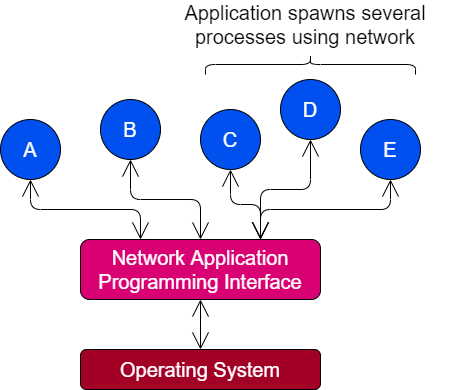
\includegraphics[width=0.6\textwidth]{the_web/images/processes.png}\end{center}
Two communicating processes the roles:
\\
\\ \begin{minipage}[t]{0.48\textwidth}
    \centerline{\textbf{Client}}
    \begin{itemize}
        \setlength\itemsep{0em}
        \item Initiates communications.
        \item If on a connection-oriented service, the client establishes the connection.
    \end{itemize}

    When using sockets:
    \begin{enumerate}
        \setlength\itemsep{0em}
        \item Creates a socket $C$ by connecting to server (e.g to host $H$ on port $P$).
        \item Use socket $C$ by writing/reading to/from it (body of client app protocol).
        \item Disconnect and destroy the socket.
    \end{enumerate}
\end{minipage}
\hfill
\begin{minipage}[t]{0.48\textwidth}
    \centerline{\textbf{Server}}
    \begin{itemize}
        \setlength\itemsep{0em}
        \item Waits for connections.
        \item If on a connection-oriented service, the server passively accepts connection requests.
    \end{itemize}
    When using sockets:
    \begin{enumerate}
        \setlength\itemsep{0em}
        \item Create a server socket $S$ by accepting a connection on port $P$
        \item Read/Write data from socket to use it (body of server app protocol).
        \item Disconnect and destroy $S$.
    \end{enumerate}
\end{minipage}
\begin{sidenotebox}{Peer-to-Peer}
    In \textbf{Peer-to-Peer} (P2P) networking both processes act as both clients and servers. For example BitTorrent ($\mu Torrent$), Gnutella, even Skype and Spotify for some time.
\end{sidenotebox}
\begin{sidenotebox}{World Wide Web}
    Based on concepts of \textbf{hypertext} and \textbf{hyperlinks}.
    \begin{itemize}
        \setlength\itemsep{0em}
        \item Basically glorified FTP, transferring plain text.
        \item HTTP and old concept (based on proposal by William Tunnicliffe in the 60s).
        \item HTML language is very simple.
        \item HTTP protocol is stateless \& simple.
        \item Low barrier of entry to learn and use.
        \item GUI browsers make it more accessible, 3rd party graphical applications appreciate the ecosystem.
    \end{itemize}
\end{sidenotebox}

\section{Web Terminology}
\begin{center}
    \begin{tabular}{l p{0.9\textwidth}}
        \textbf{document}   & A webpage, a website containing several.                                              \\
        \textbf{objects}    & A file, a document may contain several (HTML, JS, video, images).                     \\
        \textbf{URL}        & Uniform Resource Locator (specifies the address of an object).                        \\
        \textbf{browser}    & Program to request, receive document and process the document to display graphically. \\
        \textbf{web server} & An application containing document and objects, serving them to clients over HTTP.    \\
    \end{tabular}
\end{center}
\begin{definitionbox}{HTTP}
    HyperText Transfer Protocol used fro transfering web objects. It uses a connection-oriented mechanism (\textbf{TCP}) but can also work over connectionless (e.g \textbf{UDP}).
    \begin{itemize}
        \setlength\itemsep{0em}
        \item Each request and repsonse is a single unit.
        \item No request depends on a previous one (stateless), everything is self contained.
        \item If a request is dropped, others are not affected.
    \end{itemize}
    \[\begin{matrix}
            HTTP/1.0 & HTTP/1.1 & HTTP/2.0 & HTTP/3
        \end{matrix}\]
    $1.1$ is the most popular, with $2.0$ being faster and influenced by projects at google. $3$ is in final draft.
    \\
    \\ $80$ is the port for HTTP requests.
\end{definitionbox}
\section{HTTP Connections}
\subsection{HTTP/1.0}
Used one \textbf{TCP} connection per object. This is inefficient and requires may objects to be spawned and destroyed.
\subsection{HTTP/1.1}
\begin{itemize}
    \setlength\itemsep{0em}
    \item Same \textbf{TCP} connection is used to issue multiple requests and receive multiple responses (can receive multiple objects).
    \item Default behaviour is to use persistent connections (keep open to send further requests).
    \item Request containing $Connection: \ close$ closes the connection, done after all responses/requests have been sent.
\end{itemize}

\subsection{HTTP/2}
Expected to replace HTTP/1.x completely within a few years.
\begin{itemize}
    \setlength\itemsep{0em}
    \item Exchanges content in binary, allowing for more compact representation and higher speed (less data to transfer).
    \item Connection is fully multiplexed (not ordered or blocking)
    \item Can use a single \textbf{TCP} connection with requests in parallel.
\end{itemize}

\subsection{HTTP/3}
Uses \textbf{UDP} for exchanges (faster).
\subsection{Persistent Connections}
\begin{center}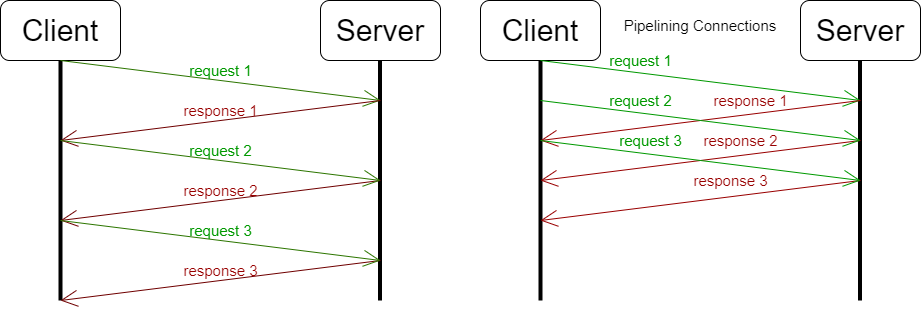
\includegraphics[width=0.8\textwidth]{the_web/images/requests.png}\end{center}
\subsection{Protocol Features}
\twosplit{
    \textbf{Request}
    \begin{itemize}
        \setlength\itemsep{0em}
        \item Protocol Version
        \item URL Specification
        \item Connection Attributes
        \item Content/Feature Negotiation
    \end{itemize}
}{
    \textbf{Response}
    \begin{itemize}
        \setlength\itemsep{0em}
        \item Protocol Version
        \item Reply Status/Value
        \item Connection Attributes
        \item Object Attributes
        \item Content Specification (type, length)
        \item Content (objects)
    \end{itemize}
}
\subsection{HTTP Methods}

\begin{tabular}{l p{.8\textwidth}}
    \textbf{GET}  & retrieve object using \textbf{URL}.                                    \\
    \textbf{POST} & Submit data to server (e.g a form, message).                           \\
    \textbf{HEAD} & Like get, but only receive the header, used for testing link validity. \\
\end{tabular}

\subsection{Anatomy of a Response}
\inputminted{HTML}{the_web/code/response.html}
\begin{definitionbox}{Status Code}
    A 3 digit code:
    \begin{center}
        \begin{tabular}{l p{0.9\textwidth}}
            $1xx$ & Informational.                                                                                                            \\
            $2xx$ & Successful Operation (e.g $200 \to OK$).                                                                                  \\
            $3xx$ & Redirection (object has moved either temporarily or permanently).                                                         \\
            $4xx$ & Client Error,  e.g $400$ (Malformed Request), $401$ (Unauthorized), $404$ (Object not found), $405$ (Method not allowed). \\
            $5xx$ & Server error, e.g $500$ (internal server error), $503$ (service overloaded).                                              \\
        \end{tabular}
    \end{center}
\end{definitionbox}

We can use \fun{telnet} to send plain-text commands directly to a server listening on a specific port ($80$ for HTTP).

\inputminted{bash}{the_web/code/telnet_imperial.sh}

\section{Web Caching}
\begin{center}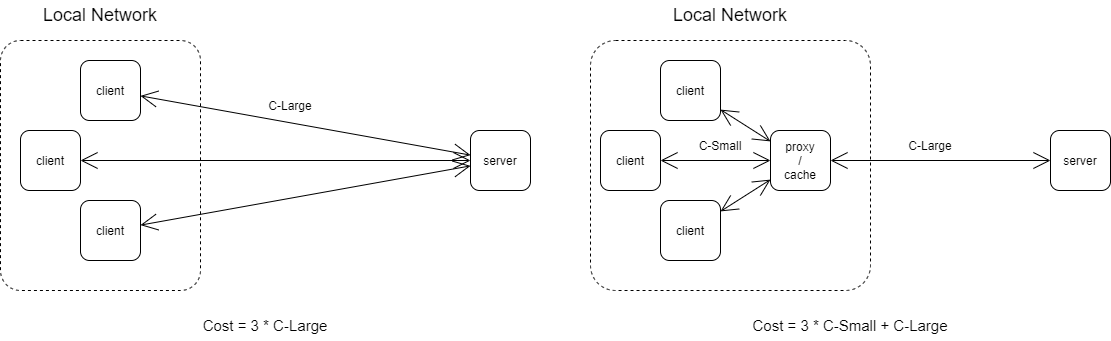
\includegraphics[width=\textwidth]{the_web/images/proxy cache.png}\end{center}
A proxy can be used to speed up common requests.

\begin{enumerate}
    \setlength\itemsep{0em}
    \item Get request from client.
    \item Check if request is cached.
    \item If cached, take cached response.
    \item If not, forward request to server acting as a client, cache the response for some time.
    \item Forward the response to the client.
\end{enumerate}

\twosplit{
    \textbf{Benefits}
    \begin{itemize}
        \setlength\itemsep{0em}
        \item Reduced latency for requests.
        \item Reduced network traffic.
        \item Better security, server only sees proxy.
        \item When using a firewall on proxy, \textbf{LAN} protected from intrusions.
    \end{itemize}
}{
    \textbf{Problems}
    \begin{itemize}
        \setlength\itemsep{0em}
        \item Latency associated with finding entries and caching.
        \item Complexity (need a proxy to be setup).
        \item Need to determine how long cache entries last for data freshness.
    \end{itemize}
}
Proxy/Cache is central to several HTTP features.
\begin{itemize}
    \setlength\itemsep{0em}
    \item HTTP is defined as a request/response protocol, where requests and responses are explicitly passed through the response chain.
    \item Explicitly specifies how protocol version are handled on the request chain.
    \item Determines how each method should be handled (e.g only cacheable if indicated by \const{Cache-Control} or \const{Expires} in the header, $OPTION$ requests are not cacheable).
    \item Cached pages can become stale. A HEAD request can be made to see if an object has been updated (and cache needs to be invalidated).
    \item Servers can specify explicit expiration times using either the \const{Expires} header, or the \var{max-age} directive of the \const{Cache-Control} header.
    \item A client or proxy can use a condition GET request including an \const{If-Modified-Since} header.
\end{itemize}
\begin{examplebox}{Requests}
    \begin{center}
        \begin{minipage}[t]{0.9\textwidth}
            \inputminted{HTML}{the_web/code/do_not_cache_requests}
        \end{minipage}
    \end{center}
\end{examplebox}
\begin{examplebox}{Responses}
    \begin{center}
        \begin{minipage}[t]{0.9\textwidth}
            \inputminted{HTML}{the_web/code/do_not_cache_responses}
        \end{minipage}
    \end{center}
\end{examplebox}

\section{HTTP Sessions}
HTTP is a stateless protocol, however we need stateful applications (e.g shopping cart for website, playlist next track identifier).
\\
\\ This is done through the \const{Set-Cookie} and \const{Cookie} headers:
\begin{center}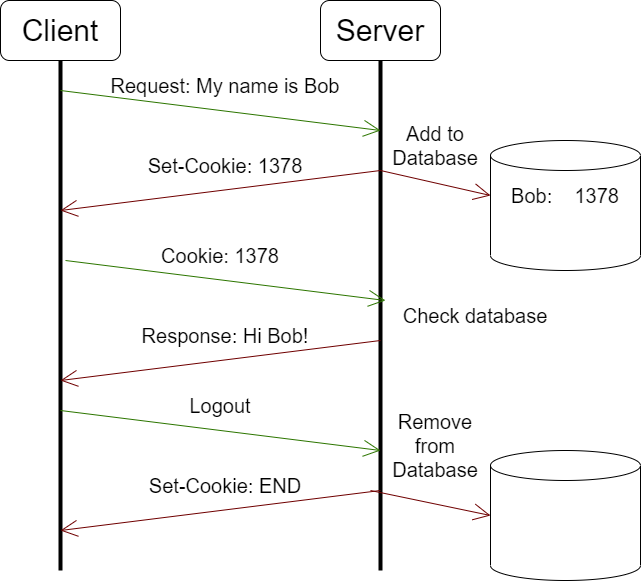
\includegraphics[width=0.6\textwidth]{the_web/images/cookies.png}\end{center}
Some websites keep cookies between visits to track users. Others only use cookies for the extent of a session (given cookie at login, cookie deleted at logout).

\section*{Dynamic Web Pages}
Instead of storing and serving static web pages, generate webpages for a given user's request (e.g chat, profile, recommendations based on account or session).
\begin{definitionbox}{Common Gateway Interface}
    Allows a program to identify parameters from the url.
    \\
    \\ https://www.mywebsite.com/page.html?name=oliver\&age=19\&day=monday
    \\
    \\ The webserver gets the request url, and can then process it in any way it chooses (e.g for non-existent pages, returning a $404$ page).
\end{definitionbox}

\begin{sidenotebox}
    A Java based solution to state, the webserver creates new instances of the JVM to run \& process requests for each client connecting.
\end{sidenotebox}

An alternative approach is to execute code on the client side. The code is sent to the clients browser to run, rather than the server creating new pages to send.
\begin{examplebox}{Javascript and PHP}
    PHP (PHP Hypertext Processor) is server side, generating pages to be sent to the client.
    \begin{center}
        \begin{minipage}[t]{0.9\textwidth}
            \inputminted{HTML}{the_web/code/php_example.html}
        \end{minipage}
    \end{center}
    Javascript is client side, the code is sent to the client (embedded in the web page) and run on the client side to create the page.
    \begin{center}
        \begin{minipage}[t]{0.9\textwidth}
            \inputminted{HTML}{the_web/code/javascript_example.html}
        \end{minipage}
    \end{center}
\end{examplebox}

\section{Domain Name System (DNS)}
\subsection{IP Addresses}
Uniquely identifies an end system by an address.
\begin{center}
    \begin{tabular}{l l l}
        \textbf{Type} & \textbf{Size}     & \textbf{Example}                 \\
        PIv4          & $32$ bit address  & $146.169.41.237$                 \\
        PIv6          & $128$ bit address & $fe80::211::43ff::fecd::30f5/64$ \\
    \end{tabular}
\end{center}
\begin{itemize}
    \setlength\itemsep{0em}
    \item Easy format for routers to process quickly.
    \item Not practical for use by people.
\end{itemize}
\begin{sidenotebox}{Pre-1983}
    Users can use a file containing mappings of host mnemonics to IP addresses.
\end{sidenotebox}

\subsection{Domain Name System}
A distributed lookup facility for mapping hostnames to IP addresses.
\begin{center}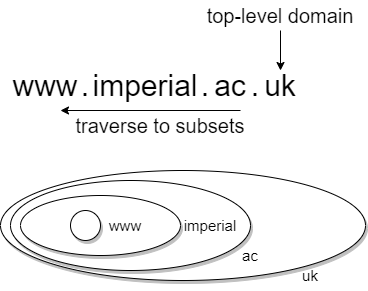
\includegraphics[width=0.6\textwidth]{the_web/images/domains.png}\end{center}
\begin{tabular}{l p{.8\textwidth}}
    \textbf{Root Servers}             & Each top-level domain (e.g .com, .edu, .org, .uk etc) is associated one of $13$ root DNS servers operated by one of $12$ independent organizations. \\
    \textbf{Top-Level Domain Servers} & A DNS server associated with a top-level domain.                                                                                                    \\
    \textbf{Authoritative Servers}    & For each domain, a server holds the master copy mapping all public hosts within that domain.                                                        \\
\end{tabular}

Most root servers as well as lower level servers are implemented as a distributed set of machines.
\\
\\ By distributing copies of DNS maps (that are constantly updated) across the world traffic can be load balanced, latency can be lower (have servers geographically near) and there is redundancy (e.g if a server is damaged or down for maintenance).
\subsection{DNS Caching}
Important to reduce the load on DNS infrastructure while improving performance.
\begin{itemize}
    \setlength\itemsep{0em}
    \item Cache can go stale, may needs to be updated from authoritative server.
    \item \textbf{DNS Cache Poisoning}
\end{itemize}

\begin{sidenotebox}{DNS Cache Poisoning}
    also called DNS spoofing, entering incorrect mappings into a DNS cache to direct users to the wrong site.
\end{sidenotebox}

\subsection{DNS Features}
DNS can be described as a directory service database. Each entry is a \textbf{Resource Record} describing a translation of a name.
\begin{center}
    \begin{tabular}{l l l l}
        \textbf{Name}       & \textbf{Value}     & \textbf{Type} & \textbf{TTL - Time to Live} \\
        www.imperial.ac.uk  & 146.179.40.148     & A             & \dots                       \\
        shell3.doc.ic.ac.uk & 146.169.21.39      & A             & \dots                       \\
        www3.imperial.ac.uk & www.imperial.ac.uk & CNAME         & \dots                       \\
        imperial.ac.uk      & ns0.ic.ac.uk       & NS            & \dots                       \\
        imperial.ac.uk      & mx1.cc.ic.ac.uk    & MX            & \dots                       \\
    \end{tabular}
\end{center}
\begin{itemize}
    \setlength\itemsep{0em}
    \item {\textbf{Time to Live}
          \\ Specifies how long the mapping should be cached before being invalidated.
          }
    \item {\textbf{Type}
          \\
          \\ \begin{tabular}{l l l l}
              \textbf{Type} & \textbf{Name}   & $\to$ & \textbf{Value}                                       \\
              A             & host name       & $\to$ & IP Address                                           \\
              NS            & domain name     & $\to$ & authoritative name server                            \\
              CNAME         & host name alias & $\to$ & primary/canonical host name                          \\
              MX            & host name       & $\to$ & server to receive incoming mail (MX - Mail eXchange) \\
          \end{tabular}
          }
\end{itemize}
More of the types can be found in the "Resource Record (RR) Types" table \href{https://www.iana.org/assignments/dns-parameters/dns-parameters.xhtml}{here}.
\subsection{DNS Protocol}
\begin{tabular}{l p{.8\textwidth}}
    \textbf{Connectionless} & Runs on top of UDP (User Datagram Protocol in the transport layer) on port $53$. This is as getting a hostname translation only requires two packets (request with name \& reply with the value), so the overhead of setting up and closing a TCP connection would be significant compared to the message time. \\
    \textbf{Messages}       & Has query and reply messages, an identifier is contained in both so messages can be associated.                                                                                                                                                                                                                 \\
    \textbf{Same format}    & Queries and Replies have the same basic format for simplicity.                                                                                                                                                                                                                                                  \\
\end{tabular}

\subsection{Round Robin DNS}
A load-balancing technique for geographically distributed web servers.
\\
\begin{enumerate}
    \setlength\itemsep{0em}
    \item DNS server requests translation of hostname from an authoritative DNS server.
    \item A DNS request (to get mapping) is responded to with a list of IP Addresses.
    \item DNS server round robins through each address (using each a specific number of times before moving to the next) to make clients send requests to many IPs.
    \item Requests to hostname balanced across many servers.
\end{enumerate}
Note that when using this technique, TTL should be low ($<18$ seconds), so that the DNS server updates its list often and hence can get the most up to date list of servers available/not snowed under with requests.
\\
\\ e.g
\begin{enumerate}
    \setlength\itemsep{0em}
    \item Send list with mapping to server A to DNS server 1.
    \item Server A becomes overloaded.
    \item DNS server 1 requests and update.
    \item New list does not contain A.
\end{enumerate}
\subsection{Manual DNS Lookup}
\begin{definitionbox}{Name Server Lookup (nslookup)}
    A tool to find DNS information for a hostname.
    \begin{center}
        \begin{minipage}[t]{0.9\textwidth}
            \inputminted{bash}{the_web/code/nslookup_example.sh}
        \end{minipage}
        \begin{itemize}
            \setlength\itemsep{0em}
            \item The first line specifies the DNS server used.
            \item Non-authoritative specifies the address was extracted from the DNS server's cache.
        \end{itemize}
        \begin{minipage}[t]{0.9\textwidth}
            \inputminted{bash}{the_web/code/nslookup_get_name_server.sh}
        \end{minipage}
    \end{center}
\end{definitionbox}
\begin{definitionbox}{Domain Information Groper (dig)}
    Provides more information on name servers.
    \begin{center}
        \begin{minipage}[t]{0.9\textwidth}
            \inputminted{bash}{the_web/code/dig_example.sh}
        \end{minipage}
    \end{center}
    Much like \fun{nslookup} \fun{dig} can query for types of DNS records.
    \begin{center}
        \begin{minipage}[t]{0.9\textwidth}
            \inputminted{bash}{the_web/code/dig_mail_exchange.sh}
        \end{minipage}
    \end{center}
\end{definitionbox}

\section{Content Delivery Networks}
When storing large files (e.g videos) there are two solutions:
\\ \twosplit{
    \textbf{Store on a single powerful server.}
    \begin{itemize}
        \setlength\itemsep{0em}
        \item If server down, the file is inaccessible.
        \item Server can over overwhelmed (run out of sockets or system resources) and become slow.
        \item Local network can become congested (switches connected to server become overwhelmed, slow donw \& drop packets).
        \item In a single location, so clients may be very far away, so latency is high.
    \end{itemize}
}{
    \textbf{Store and serve many copies from many geographically distributed servers.} (The \textbf{CDN} approach.)
    \begin{itemize}
        \setlength\itemsep{0em}
        \item Clients can be closer to servers (lower latency).
        \item Lots of redundancy.
    \end{itemize}
}
\begin{examplebox}{CDN Usage}
    Video Stored at \textit{http://CDN.com/as8f1324kje12i2}, but requested from \textit{http://notNetflix.com/coolvideo}.
    \begin{enumerate}
        \setlength\itemsep{0em}
        \item Client requests \textit{http://CDN.com/as8f1324kje12i2} from local DNS to get $172.24.128.1$.
        \item Client connects to $172.24.128.1$ over HTTP to get web page.
        \item Web page is received, it contains a video at address \textit{http://CDN.com/as8f1324kje12i2}.
        \item Client requests \textit{http://CDN.com/as8f1324kje12i2} from local DNS.
        \item Local DNS has authoritative DNS stored (CDN's DNS), so connects to CDN's DNS.
        \item CDN's DNS uses the local DNS' location, determines which server to connect, and the IP of the video on that server: $142.25.228.77$.
        \item Client connects to $142.25.228.77$ to get video, streams over HTTP.
    \end{enumerate}
\end{examplebox}

\subsection{Main CDN approaches}
\twosplit{
    \centerline{\textbf{Enter Deep}}
    Place CDN servers inside many access networks (e.g inside ISP's own networks).
    \begin{itemize}
        \setlength\itemsep{0em}
        \item Very close to users, so low latency.
        \item Very large number of servers to maintain on many sites.
        \item Need to get access to other organisation's networks.
    \end{itemize}
    \begin{sidenotebox}{Akamai}
        A large \textbf{CDN} network using the "enter deep" approach. According to their \href{https://www.akamai.com/company/facts-figures}{website} $85\%$ of the worlds internet users are within a single hop of an \textbf{Akami} \textbf{CDN} server.
    \end{sidenotebox}
}{
    \centerline{\textbf{Bring Home}}
    Place a smaller number of CDN servers in large clusters at \textbf{Pop} (point of Presence) locations very close to, but not inside, access networks.
    \begin{sidenotebox}{Limelight}
        A very large CDN using the "bring home" appraoch. Their private network extends globally to connect to thousands of ISPs. According to their \href{https://www.limelight.com/orchestrate-platform/global-infrastructure/}{website} they have $123$ points of presence.
    \end{sidenotebox}
}
\subsection{CDN Performance}
To lower latency, the CDN Node (server) used must be the closest to the client requesting the resource.
\begin{itemize}
    \setlength\itemsep{0em}
    \item CDN will only see the local DNS server's address (difficult to use).
    \item As a result for some \textit{faster} DNS services such as google's or cloudflare's CDNs will often pick sub-optimal nodes.
\end{itemize}

Alternatively the client can be given a list of \textbf{CDN} servers, it can then pick the best (by pinging to get latency) \& then choose the best (this is the approach used by Netflix).
\begin{sidenotebox}{Netflix}
    Originally on Amazon Web Services, but now on their own \textbf{CDN}. They use a hybrid between the "bring home" and "enter deep" approaches.
\end{sidenotebox}

\section{Email}
\begin{definitionbox}{Email}
    Text based (with attachments) communication:
    \begin{tabular}{l p{.8\textwidth}}
        \textbf{Asynchronous}          & Can send messages to users when they are offline.                                                \\
        \textbf{One-to-Many}           & Can send the same email to many recipients.                                                      \\
        \textbf{Multimedia}            & Can attach small files such as images or video.                                                  \\
        \textbf{No Authentication}     & Messages can be forged or modified.                                                              \\
        \textbf{No Confidentiality}    & Plain text that can be read by snoopers.                                                         \\
        \textbf{No delivery Guarentee} & Can be accidentally dropped or intentionally blocked, no reliable system to acknowledge receipt. \\
    \end{tabular}
\end{definitionbox}

\begin{center}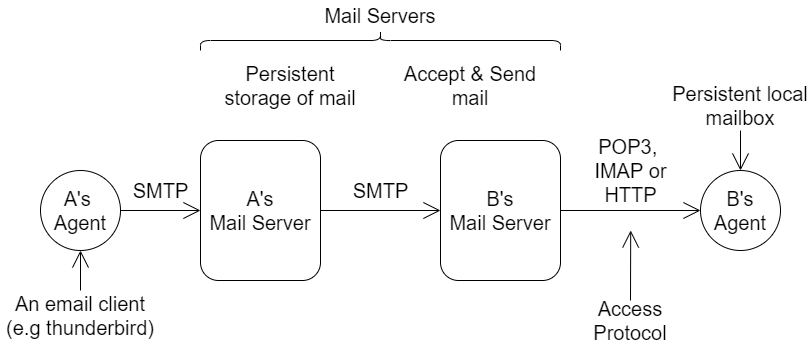
\includegraphics[width=0.8\textwidth]{the_web/images/email route.png}\end{center}
\begin{center}
    \begin{tabular}{l p{0.9\textwidth}}
        \textbf{User Agent}   & Allows users to read, compose, reply to, forward and save messages. Can often offer searching and sorting features, as well as multiple mailbox management. \\
        \textbf{Mail Servers} & { Accepts messages for remote (sending) and local (receiving) delivery.
                \begin{itemize}
                    \setlength\itemsep{0em}
                    \item Has persistent storage of remote delivery messages in a queue.
                    \item Messages for local delivery persistently stored upon receipt.
                    \item user agents can access local mailbox through \textit{access protocol}.
                \end{itemize}
        }                                                                                                                                                                                   \\
    \end{tabular}
\end{center}
Address is found using \textbf{DNS}, the MX type is for mail exchange addresses.

\subsection{Simple Mail Transfer Protocol (SMTP)}
A very simple (and old) protocol working using TCP connections on port 25.
\begin{itemize}
    \setlength\itemsep{0em}
    \item {\textbf{Simple}
          \begin{enumerate}
              \setlength\itemsep{0em}
              \item Set up TCP/IP connection from client to server.
              \item Client requests server to accept messages.
              \item Server responds, if accepting, client sends message.
          \end{enumerate}
          }
          \item{\textbf{Restrictive}
                      \\ Lines must be $\leq 1000$ characters and only supports ASCII ($7$ bit characters) (this has been fixed with extensions).
                }
          \item{ \textbf{Insecure}
                      \\ As it is very simple, so easily spoofable and can be used by malicious parties.
                }
\end{itemize}
\begin{center}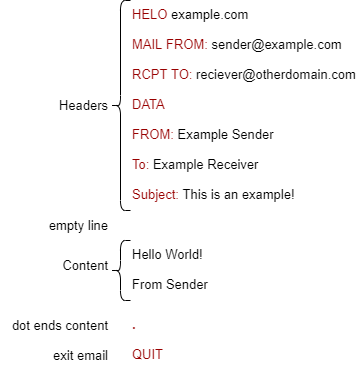
\includegraphics[width=0.6\textwidth]{the_web/images/SMTP format.png}\end{center}
\begin{sidenotebox}{Single dot emails}
    As a "." is used to terminate the email, and this is a trext character.
    \\
    \\ For each line, if the first character is a "." another is prepended to the line.
    \\
    \\ When recieving, a line with a single "." is considered terminating, otherwise if the line contains a "." followed by other characters, the "." is removed.
    \\
    \\ e.g:
    "." $\to$ \begin{tabular}{l}
        "\textcolor{red}{.}." \\
        "\textcolor{red}{.}"  \\
    \end{tabular} $\to$ \begin{tabular}{l}
        "."                  \\
        "\textcolor{red}{.}" \\
    \end{tabular} $\to$ "."
\end{sidenotebox}
\subsection{SMTP Email Headers}
\begin{center}
    \begin{tabular}{l p{0.9\textwidth}}
        \textbf{To}          & Email address/es of main destination/s.                         \\
        \textbf{Cc}          & (Carbon Copy) send copies to addresses.                         \\
        \textbf{Bcc}         & (Blind Carbon Copy) send blind copies (cannot see other Bcc'd). \\
        \textbf{From}        & Name of sender/s.                                               \\
        \textbf{Sender}      & Email address of sender.                                        \\
        \textbf{Received}    & Added by transfer agent when being received by mail server.     \\
        \textbf{Return-path} & Return address.                                                 \\
        \textbf{Date}        & Date and time the email was sent.                               \\
        \textbf{Subject}     & Short summary of the message.                                   \\
        \textbf{Reply-To}    & Email address to send replies to (typically the sender).        \\
    \end{tabular}
\end{center}
\begin{sidenotebox}{Sender}
    Often the same as "Reply-To", so usually can be left out.
\end{sidenotebox}
\textbf{SMTP} does not process message content, and should only add the "Recieved" header.
\subsection{Extensions}
\begin{tabular}{l p{.8\textwidth}}
    \textbf{SMTPS} & {\textbf{SMTP}-\textbf{S}ecure \textbf{SMTP} is plain-text, \textbf{SMTPS} adds encryption (\textbf{TSL/SSL}).
            \newline
    \newline Uses \const{STARTTLS} as the start word instead of \const{HELO}. This can be done over the same port ($25$) though some servers use different \href{https://www.mailgun.com/blog/which-smtp-port-understanding-ports-25-465-587/}{ports}}                                                                                                                                                                                                                                 \\
    \textbf{ESMTP} & {\textbf{E}xtended \textbf{SMTP}. Adds more methods for XML, html and images. These can be found \href{https://www.iana.org/assignments/mail-parameters/mail-parameters.txt}{here}.  \newline \newline Uses \const{EHLO} as the start word rather than \const{HELO}. If the reciever responds in the correct way you can use \textbf{ESMTP}'s extra methods, else you can fall back to \textbf{SMTP} and send a \const{HELO}, or the server will disconnect you.} \\
    \textbf{MIME}  & {\textbf{M}ultipurpse \textbf{I}nternet \textbf{M}ail \textbf{E}xtensions. Can use provided methods to encode non-ascii as ascii characters to send over \textbf{SMTP}.
            \newline
            \newline \textbf{MIME} types include:
            \begin{tabular}{l p{.6\textwidth}}
                \textbf{text/plain}      & Normal plaintext.                   \\
                \textbf{text/html}       & A HTML-Formatted Message.           \\
                \textbf{image/jpeg}      & Message contains only an image.     \\
                \textbf{multipart/mixed} & Message consists of multiple parts. \\
            \end{tabular}
    }                                                                                                                                                                                                                                                                                                                                                                                                                                                                                  \\
\end{tabular}

\subsection{POP3}
\textbf{Post Office Protocol} 3, used to retrieve emails from the mail server.
\begin{itemize}
    \setlength\itemsep{0em}
    \item Can do basic mail retrieval.
    \item Implicitly assumes retreived mail is deleted from mails server.
    \item Uses port $110$ (unencrypted) or $995$ (\textbf{POP3S} - encrypted).
\end{itemize}
\subsection{IMAP}
\textbf{Internet Message Access Protocol}, it replaces \textbf{POP3}.
\begin{itemize}
    \setlength\itemsep{0em}
    \item Mail is kept on the server, and read online.
    \item Allows for multiple mailboxes, backed up by the ISP.
    \item Gives user control over downloading mail.
    \item Can be encrypted (\textbf{IMAPS} port $993$) or unencrypted (port $143$, rarely used).
\end{itemize}

\section{Other Protocols}
\begin{tabular}{l l p{.8\textwidth}}
    \textbf{FTP}    & File Transfer Protocol              & For exchanging files across the network. Can be combined with \textbf{SSL} encryption (\textbf{FTPS}).                                                 \\
    \textbf{SSH}    & Secure Shell                        & Direct encrypted communication, can also be used to transfer files (\textbf{SFTP}).                                                                    \\
    \textbf{Telnet} &                                     & Plain text direct communication for non-sensitive data exchange.                                                                                       \\
    \textbf{Crypto} &                                     & Protocols such as \textbf{Bitcoin Protocol} \textbf{(BP)} and \textbf{Lightning Network Protocol} (\textbf{LNP}) are becoming more used and supported. \\
    \textbf{SNMP}   & Simple Network Management Protocol  & Administrator management of network and its devices.                                                                                                   \\
    \textbf{NFS}    & Network FIle System                 & Developed by Sun (bought by oracle), enables file access over a network.                                                                               \\
    \textbf{DHCP}   & Dynamic Host COnfiguration Protocol & Allows all networked devices to get an \textbf{IP} address.                                                                                            \\
    \textbf{IRC}    & Internet Relay Chat                 & A live chat system for chatrooms designed in $1988$, now rarely used.                                                                                  \\
\end{tabular}

\begin{sidenotebox}{Tor}
    \textit{"The onion router"}, using layers of encryption to enforce anonymity online. A basic explanation is \href{https://www.youtube.com/watch?v=QRYzre4bf7I}{here}.
\end{sidenotebox}
